\maketitle

Due: Wednesday, January 24 at 11:59 pm.

This is a survey. Please answer honestly! Typing your answers is highly recommended. This homework is graded on completion. Note: There are some questions on the next page as well.

\begin{question}
  What year of college are you in, and what is your major and/or minor?
\end{question}

\begin{question}
  What is your previous mathematical experience? (Classes, extracurriculars, etc\ldots)
\end{question}

\begin{question}
  Have you studied multivariable calculus before? What multivariable topics do you already know?
\end{question}

\begin{question}
  What is your favorite piece of math? (Favorite proof, favorite problem, etc\ldots) It does not have to be related to multivariable calculus or even calculus.
\end{question}

\begin{question}
  What is your least favorite part of math?
\end{question}

The following questions' purpose is to help me pace lectures accurately. None of these are by any means a prerequisite for this class.

\begin{question}
  Does the notation $\{(x,y,z)\in\bR^3\mid 0\leq x\leq 1, 0\leq y\leq 2, 0\leq z\leq 3\}$ mean anything to you? If it does, try to describe what it depicts in words.
\end{question}
\begin{solution}
  The braces in $\{(x,y,z)\in\bR^3\mid 0\leq x\leq 1, 0\leq y\leq 2, 0\leq z\leq 3\}$ indicate that we are talking about a set. To the left of the vertical bar is the type of elements that the set consists of, and to the right of the vertical bar is the conditions for said element to be in the set.

  The notation $\bR^3$ means the set of triples of real numbers, i.e.\ the set of vectors in 3-dimensional space.

  In words, the notation translates to ``the set of vectors $(x,y,z)$ in $\bR^3$ such that $x$ is between 0 and 1, $y$ is between 0 and 2, and $z$ is between 0 and 3''.

  Hence geometrically this is a rectangular prism with sides of length 1, 2, and 3, and one corner at the origin. More specifically the notation means the set of points inside or on this rectangular prism.
\end{solution}

\begin{question}
  Let $A$ be the set of pairs of real numbers $(x,y)$ such that $x+y=0$, and let $B$ be the set of pairs of real numbers $(x,y)$ such that $x-y=0$. Can you describe what $A\cap B$ (the intersection of $A$ and $B$) looks like? What about $A\cup B$ (the union)? You can say if you have no idea or if you don't understand this question.
\end{question}
\begin{solution}
  $A\cap B$ is the set of pairs $(x,y)$ satisfying both conditions $x+y=0$ and $x-y=0$. There is only one solution: $(0,0)$. Hence $A\cap B=\{(0,0)\}$.

  A$\cup B$ is the set of pairs $(x,y)$ satisfying either $x+y=0$ or $x-y=0$, in other words, $y=-x$ or $y=x$. Not much else can be said after that, but perhaps a picture will help:
  \begin{center}
    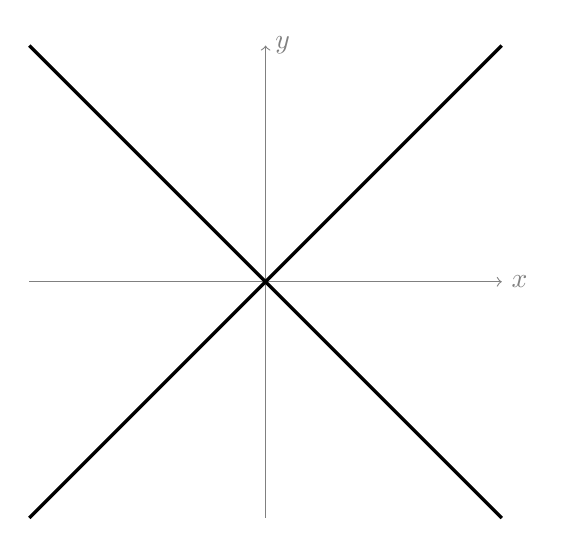
\begin{tikzpicture}
      % axes
      \draw[->, gray] (-3,0) -- (3,0) node[right]{$x$};
      \draw[->, gray] (0,-3) -- (0,3) node[right]{$y$};

      % draw the lines x=y and x=-y
      \draw[very thick] (-3,-3) -- (3,3);
      \draw[very thick] (-3,3) -- (3,-3);

    \end{tikzpicture}
  \end{center}
\end{solution}

\begin{question}
  Do you know what a partial derivative is? It's okay if you don't -- it's one of the topics for this class. What do you know about it?
\end{question}
\begin{solution}
  The partial derivative of a multivariable function is the derivative of the function with respect to one variable, holding other variables constant. (We'll visit this concept soon!)
\end{solution}

\begin{question}
  Consider the following integral:
  \[\int_1^2\int_1^2 xy\,dx\,dy.\]
  Is this something you feel you can evaluate with your current level of knowledge, or do you feel like you need to learn some multivariable calculus to evaluate this integral?
\end{question}
\begin{solution}
  This integral is indeed solvable with your current knowledge. It's just an integral of an integral. We simplify the inner integral first. The computation goes like this:
  \[\begin{split}
    \int_1^2\int_1^2 xy\,dx\,dy &= \int_1^2\left(\int_1^2 xy\,dx\right)\,dy \\
    &= \int_1^2 \left[ \frac 12 y x^2 \right]_1^2\,dy \\
    &= \int_1^2 \left(\frac 32y\right)\,dy\\
    &= \frac 34y^2\Big|_1^2\\
    &= \frac 94.
  \end{split}\]
  When computing the inner integral, in the first line, $y$ is treated like a constant.
\end{solution}

\begin{question}
  Is the following sentence true or false?
  \[\lim_{a\to\infty}\int_{-a}^a x^3\,dx\text{ diverges}.\]
  You can say ``not sure'' if you're not sure.
\end{question}
\begin{solution}
  False. Like the previous expression, we simplify the expression inside out. The expression inside the limit is a definite integral which evaluates to 0 no matter what $a$ is. Therefore, the limit is computing the limit of the constant function 0 as $a\to\infty$, which is 0.
\end{solution}

\begin{question}
  Have you ever seen a mathematical proof, outside of two-column proofs? Have you seen one you thought was nice or elegant? Briefly describe anything you remember about it if so.
\end{question}
\begin{solution}
  Some of the elegant proofs you've mentioned include, off the top of my head:
  \begin{itemize}
    \item A proof that $0.999\ldots=1$.
    \item Some proofs of the Pythagorean theorem.
    \item The proof that $\sqrt2$ is irrational.
    \item Some examples of proof by induction, including one that shows that the sum of the first $n$ odd numbers is equal to $n^2$.
  \end{itemize}
  These are great. On the other hand, I know this class is the first exposure to proofs (let alone elegant ones) for many of you. I hope to present every proof in this course as elegantly as possible!
\end{solution}

\begin{question}
  This is the counterpart to the previous question. Do you feel proofs are scary? Are you scared about the prospects of proofs being involved in this course?
\end{question}
\begin{solution}
  I hope by the end of this course you see that proofs are nice, rather than scary or tedious :)
\end{solution}
